\documentclass[11pt,a4paper]{article}
\usepackage{color}
\usepackage{enumitem}
\usepackage{fullpage}
\usepackage{graphicx}
\usepackage[colorlinks=true, linkcolor=blue]{hyperref}
\usepackage{listings}

\newcommand{\FSharp}{{\settoheight{\dimen0}{F}F\kern-.05em \resizebox{!}{\dimen0}{\raisebox{\depth}{\#}}}}

\definecolor{bluekeywords}{rgb}{0.13,0.13,1}
\definecolor{greencomments}{rgb}{0,0.5,0}
\definecolor{redstrings}{rgb}{0.5,0,0}

\lstdefinelanguage{FSharp}
{
	morekeywords={let, new, match, with, rec, open, module, namespace, type, of, member, and, for, in, do, begin, end, fun, function, try, mutable, if, then, else},
	keywordstyle=\color{bluekeywords},
	sensitive=false,
	morecomment=[l][\color{greencomments}]{//},
	morecomment=[s][\color{greencomments}]{{(*}{*)}},
	morestring=[b]",
	stringstyle=\color{redstrings},
	basicstyle=\ttfamily,
	breaklines=true,
	columns=fullflexible
}

\begin{document}
\title{Implementing a Simple Logic Inference Engine in \FSharp}
\author{Libo Yin, 2116 4183\\The University of Western Australia}
\maketitle

\section{High-Level Strategy}

The problem solving process is modeled as a depth-first search tree. In contrast to a traditional search tree, this tree has following properties:

\begin{enumerate}[itemsep=0mm]
\item There are two types of nodes: \texttt{QUERY} nodes and \texttt{RULE} nodes
\item There are two types of edges: \texttt{AND} edges and \texttt{OR} edges.
\item A \texttt{QUERY} node is branched to \texttt{RULE} nodes through \texttt{OR} edges. A \texttt{QUERY} node succeeds if \emph{any} of its children \texttt{RULE} nodes succeeds.
\item A \texttt{RULE} node is branched to \texttt{QUERY} nodes though \texttt{AND} edges. A \texttt{RULE} node succeeds if it can be applied to its parent \texttt{QUERY} node, and \emph{all} of its children \texttt{QUERY} nodes succeeds.
\item An empty \texttt{QUERY} node succeeds.
\item The root of the tree is a \texttt{QUERY} node.
\end{enumerate}

With a more problem-specific terminology, a node in the search tree is a \texttt{sufficency} in type definition: \texttt{\textcolor{blue}{type} rule = Rule \textcolor{blue}{of} sufficency * (sufficency list)}. A \texttt{RULE} node corresponds to the former one, i.e.\ the goal, while its children \texttt{QUERY} node corresponds to the latter one, i.e.\ the subgoals. A \texttt{sufficency} is satisfied if it can be unified with the goal of \emph{any} rules, and satisfy \emph{all} subgoals of that rule.

\hyperref[fig:ex1]{Figure~\ref{fig:ex}} shows an examplary search tree of query: \texttt{Mix(A,A)$\rightarrow$Mix(B,B)} using rule set: \texttt{x$\rightarrow$x if [], A$\rightarrow$B if [], Mix(x1,x2)$\rightarrow$Mix(y1,y2) if [x1$\rightarrow$y1,x2$\rightarrow$y2]}.

\begin{figure}[htbp]
	\centering
	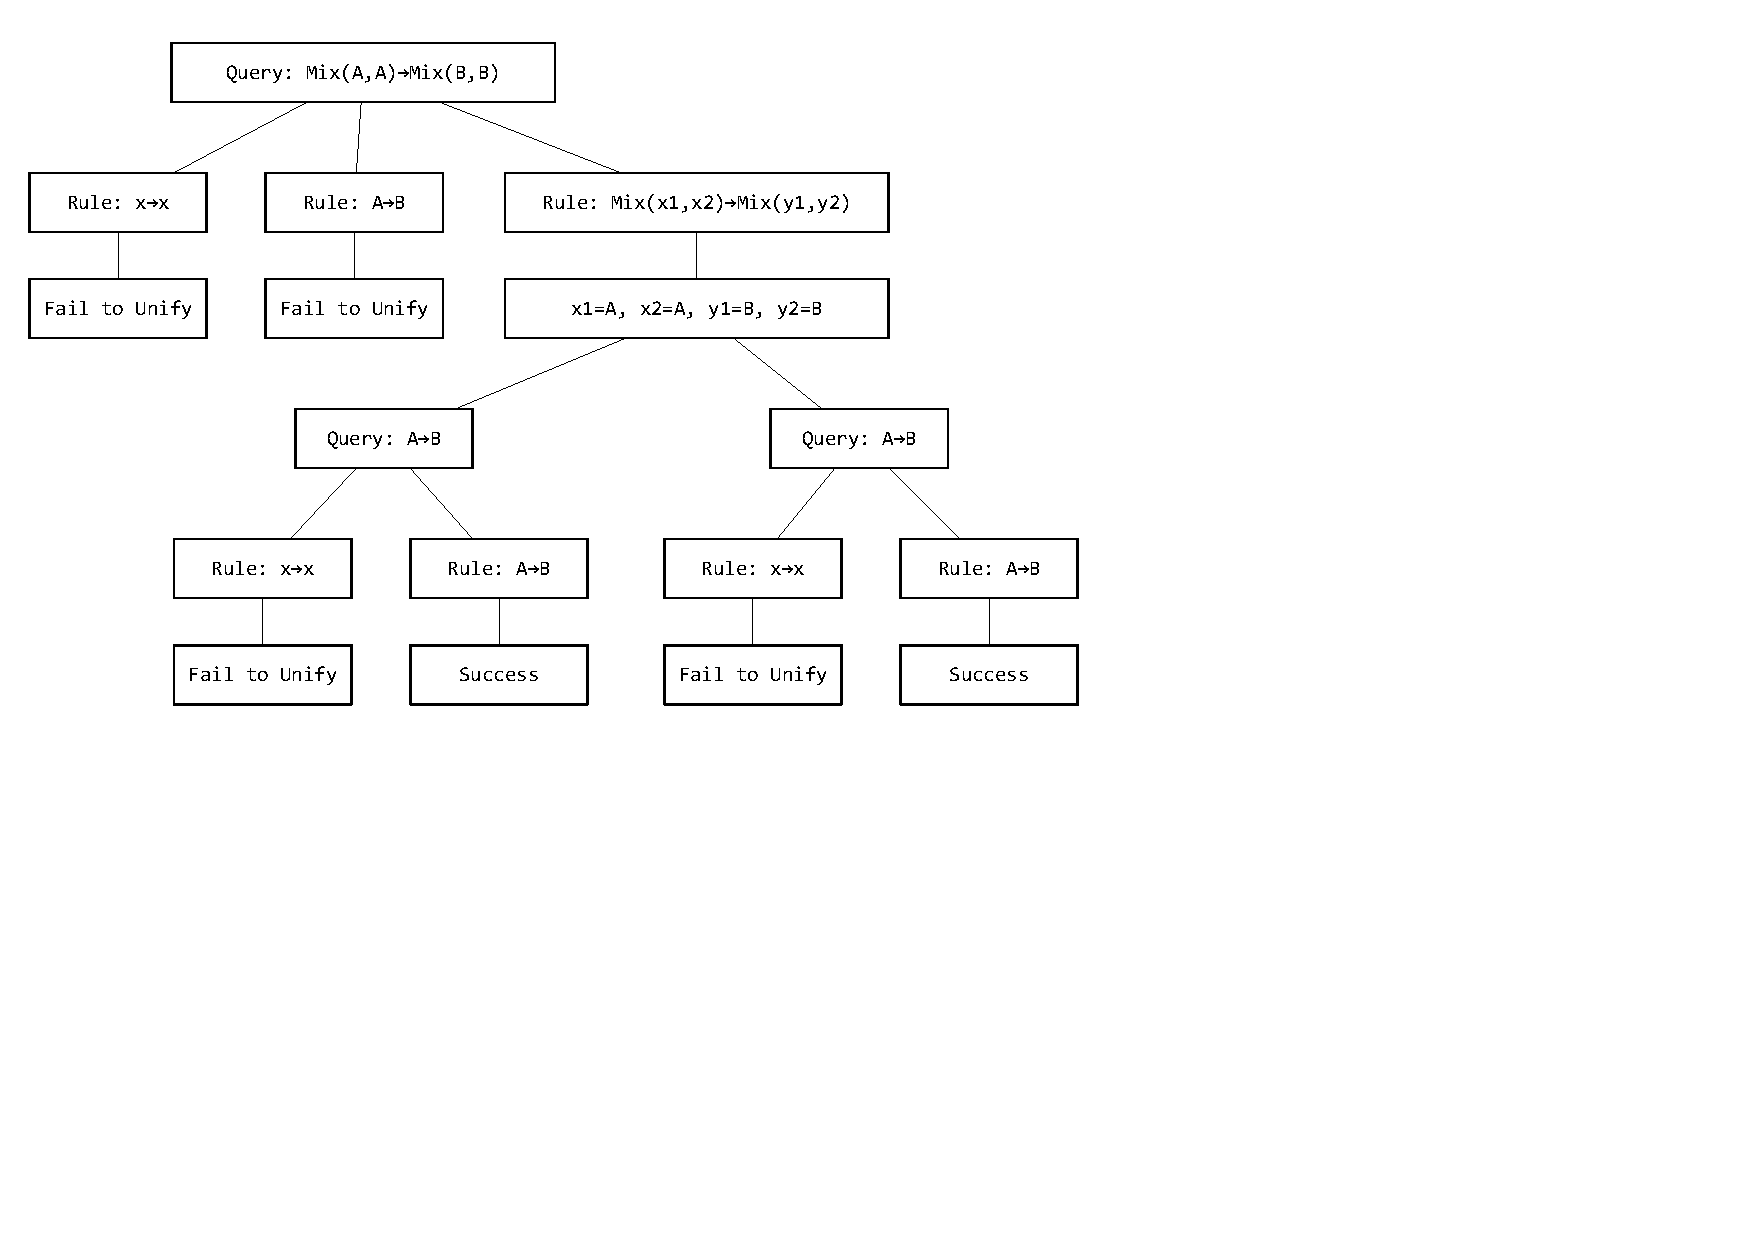
\includegraphics[scale=0.8]{search_tree.pdf}
	\caption{Examplary search tree of query: \texttt{Mix(A,A)$\rightarrow$Mix(B,B)} using rule set: \texttt{x$\rightarrow$x if [], A$\rightarrow$B if [], Mix(x1,x2)$\rightarrow$Mix(y1,y2) if [x1$\rightarrow$y1,x2$\rightarrow$y2]}.}
	\label{fig:ex}
\end{figure}

\section{Handling Unknowns}

One distinct feature of logical programming is the existence of unknowns. Unknowns may appear in rules and queries, and may refer to expressions that either have already appeared before, or will only be known later. Unknowns are handled with the classic approach of unification, i.e.\ association of unknowns to known expressions. To assist the unification function, the concept of dictionary is introduced.

Dictionary is the cumulative result of successful unifications, containing mappings from unknowns to stable expressions. A stable expression is defined as a known expression, an unknown that is not in the dictionary, or a combination of stable expressions.

Dictionary is used in unification twice. Prior to the unification, a dictionary lookup is performed on each of the two expressions to be unified, reducing the number of unknowns. After the unification, new mappings are added to the dictionary. If the unification fails, no change is made to the dictionary.

Another issue concerning unknowns is that the same rule can be applied to different queries at different depths of the search tree. In such occations, the same unknown may refer to different expressions. This problem is solved by normalizing name of unknowns: Before unification, the current depth in the search tree is appendeded to the end of all unknowns in a rule.

\section{Program Structure}

A state in the solution process is defined as a 4-tuple \texttt{dictionary * queries * rules * depth}. \texttt{Queries} is a list containing all unsolved \texttt{QUERY} nodes of their parent \texttt{RULE} node. Likewise, \texttt{rules} is a list containing all unsolved \texttt{RULE} nodes of their parent \texttt{QUERY} node. Since a \texttt{QUERY} node branches through \texttt{OR} edges, an empty \texttt{rules} indicates the failure of its \texttt{QUERY} parent. On the other hand, since a \texttt{RULE} node branches through \texttt{AND} edges, an empty \texttt{queries} indicates the success of its \texttt{RULE} parent.

If neither \texttt{queries} nor \texttt{rules} is empty, the heads of them are taken as the current query and rule. The current rule is then normalized into a 2-tuple \texttt{goal * subgoals}. Afterwards, the current query is unified with the current goal. If the unification succeeds, which means an augmented dictionary is returned, the current subgoals are solved recursively with the augmented dictionary and all rules. If \emph{all} subgoals succeed, the current query succeeds, and the solver continues with the tail of \texttt{queries}, the augmented dictionary, and all rules. On the other hand, if \emph{any} subgoal fails, or if the unification fails, the solver tries to solve the current query again with other rules, i.e.\ the tail of \texttt{rules}, and the original dictionary.

\newpage

\appendix

\section{Uncommented Source Code}

Please refer to the source code submission for commented source code.

\begin{lstlisting}[language=FSharp,numbers=left,xleftmargin=3em]
let rec MapVar (dict:Map<string,exp>) e =
    match e with
    | A | B -> e
    | Mix(e1,e2) -> Mix(MapVar dict e1, MapVar dict e2)
    | Var(key) ->
        match dict.TryFind key with
        | Some(value) -> if value=e then e else MapVar dict value
        | None -> e

let rec Contains e vn =
    match e with
    | A | B -> false
    | Mix(e1,e2) -> Contains e1 vn || Contains e2 vn
    | Var(vn') -> vn=vn'

let rec UnifyExp dict e1 e2 =
    let (x1,x2) = (MapVar dict e1,MapVar dict e2)
    match (x1,x2) with
    | _ when x1=x2 -> Some(dict)
    | (Var(vn),e) | (e,Var(vn)) ->
        if Contains e vn then None else Some(dict.Add(vn,e))
    | (Mix(e1a,e1b),Mix(e2a,e2b)) ->
        match UnifyExp dict e1a e2a with
        | Some(dict') -> UnifyExp dict' e1b e2b
        | None -> None
    | _ -> None

let UnifySuff dict s1 s2 =
    match UnifyExp dict (fst s1) (fst s2) with
    | Some(dict') -> UnifyExp dict' (snd s1) (snd s2)
    | None -> None

let rec NormExp n e =
    match e with
    | A | B -> e
    | Mix(e1,e2) -> Mix(NormExp n e1, NormExp n e2)
    | Var(vn) -> Var(vn + string n)

let NormSuff n suff = (NormExp n (fst suff),NormExp n (snd suff))

let NormRule n (Rule(goal,subgoals)) =
    (NormSuff n goal,List.map (NormSuff n) subgoals)
\end{lstlisting}

\newpage

\begin{lstlisting}[language=FSharp,numbers=left,firstnumber=43,xleftmargin=3em]
let rec Solve ar dict queries rules depth =
    if depth=8 then false else
    match queries with
    | [] -> true
    | query::qTail ->
        match rules with
        | [] -> false
        | rule::rTail ->
            let (goal,subgoals) = NormRule depth rule
            match UnifySuff dict query goal with
            | Some(dict') ->
                if Solve ar dict' subgoals ar (depth+1)
                then Solve ar dict' qTail ar depth
                else Solve ar dict queries rTail depth
            | None -> Solve ar dict queries rTail depth

let suffices ruleGens (exp1,exp2) =
    let rules = List.map (fun f -> f()) ruleGens
    Solve rules (Map.empty<string,exp>) [(exp1,exp2)] rules 0
\end{lstlisting}

\end{document}